%\title{LaTeX Portrait Poster Template}
%%%%%%%%%%%%%%%%%%%%%%%%%%%%%%%%%%%%%%%%%
% a0poster Portrait Poster
% LaTeX Template
% Version 1.0 (22/06/13)
%
% The a0poster class was created by:
% Gerlinde Kettl and Matthias Weiser (tex@kettl.de)
%
% This template has been downloaded from:
% http://www.LaTeXTemplates.com
%
% License:
% CC BY-NC-SA 3.0 (http://creativecommons.org/licenses/by-nc-sa/3.0/)
%
%%%%%%%%%%%%%%%%%%%%%%%%%%%%%%%%%%%%%%%%%

% Note: template has been modified accordingly by 8th floor CFD group for FSB
% style

%-------------------------------------------------------------------------------
%   PACKAGES AND OTHER DOCUMENT CONFIGURATIONS
%-------------------------------------------------------------------------------

\documentclass[b1b,portrait]{b0poster}

%\usepackage{multicol} % Multiple columns of text side-by-side
%\columnsep=100pt % Amount of white space between the columns
%\columnseprule=3pt % Thickness of the black line between the columns

\usepackage[svgnames]{xcolor} % Specify colors by their 'svgnames', for a full
                              % list of all colors available see here:
                              % http://www.latextemplates.com/svgnames-colors

\usepackage{graphicx} % Required for including images
\graphicspath{{figures/}} % Location of the graphics files
\usepackage{booktabs} % Top and bottom rules for table
\usepackage[font=small,labelfont=bf]{caption} % Captions of tables and figures
\usepackage{amsfonts, amsmath, amsthm, amssymb} % Math fonts, symbols, etc
\usepackage{wrapfig} % Allows wrapping text around tables and figures

\usepackage{general}
\usepackage{tensorCommon}
\usepackage{tensorEquation}
\usepackage{tensorOperator}
\usepackage{finiteVolume}

\usepackage{tcolorbox}

\usepackage{epsfig}
\usepackage{epstopdf}

\newcommand{\imsize}{0.9\columnwidth}
\newcommand{\imsizeDuoF}{0.48\columnwidth}
\newcommand{\imsizeDuoS}{0.46\columnwidth}
\newcommand{\imsizeTrio}{0.32\columnwidth}

% Define blue colour from the FSB logo
\definecolor{fsbBlue}{RGB}{57,123,199}

% Tikz package to manually draw bleed marks.
% Note: bleed marks are set to 1cm in the b0poster.cls
\usepackage{tikzpagenodes}
\usetikzlibrary{calc}

% Placeholder text
\usepackage{lipsum}

% For cross-referencing
\usepackage{hyperref}

% Change default font: phv	Helvetica
\renewcommand*\sfdefault{phv}
% Set sans serif font
\renewcommand{\familydefault}{\sfdefault}

% Itemization symbols
\newcommand{\localtextbulletone}{\textcolor{fsbBlue}{\raisebox{.45ex}{\rule{.6ex}{.6ex}}}}
%\newcommand{\localtextbullettwo}{\textcolor{fsbBlue}{\raisebox{.45ex}{\rule{1.2ex}{.3ex}}}}
\renewcommand{\labelitemi}{\localtextbulletone}
%\renewcommand{\labelitemii}{\localtextbullettwo}

\begin{document}

%-------------------------------------------------------------------------------
%   POSTER HEADER
%-------------------------------------------------------------------------------

% The header is divided into two boxes:
% 1. 30% wide for UNIZAG and FSB logo with information on department
% 2. 70% wide for information regarding chair

% First box
\begin{minipage}[t][7cm][c]{0.3\linewidth}
\centering
\raisebox{-0.5\height}{
\includegraphics[width=4.5cm]{logoUNIZAG.pdf}}\hspace{1cm}
\raisebox{-0.5\height}{
\includegraphics[width=10cm]{logoFSB.pdf}}\\[0.35cm]
%\vspace{1cm}
{\small
% Department name
University of Zagreb\\
Faculty of Mechanical Engineering and Naval Architecture\\
Department of Energy, Power and Environmental Engineering%\\
%Chair of Turbomachinery
}
\end{minipage}%
%
% Second box
\fcolorbox{fsbBlue}{fsbBlue}{%
\begin{minipage}[t][7cm][c]{0.7\linewidth}
  \centering
  % Name of the chair
  {\huge\textcolor{white}{%
  \textbf{Implementation of Discontinuous Galerkin \\ in OpenFOAM}\\
  }}
\end{minipage}
}

%-------------------------------------------------------------------------------
%   TRANSITION FROM HEADER TO MAIN CONTENT
%-------------------------------------------------------------------------------

\vspace{1.6cm}

%-------------------------------------------------------------------------------
%    MAIN CONTENT
%-------------------------------------------------------------------------------

% Main content is divided into three boxes:
% 1. Left part for abstract/introduction
% 2. Middle part for main content
% 3. Right part for main content
% Note: height of minipage is hacked for B1 poster size, if other sizes are
% used, this needs to be changed.

% First box:
\fcolorbox{fsbBlue}{fsbBlue}{%
\begin{minipage}[t][79cm][t]{0.293\linewidth}
  \setlength{\baselineskip}{1.4em}
  \textcolor{white}{%
    % Author
    \begin{center}
      \LARGE \bfseries
      Hrvoje Jasak \\ Gregor Cvijeti\'{c} \\ Tessa Uroi\'{c}
    \end{center}
  % Abstract: Adjust font size to \large, \Large or \LARGE as needed
\large
\vspace{0.5 cm}
\LARGE \textit{Introduction}
\\
\large
OpenFOAM is an open source Computational Fluid Dynamics (CFD) toolbox based on
the Finite Volume Method (FVM). The advantage of FVM is a straightforward and
relatively easy formulation of equations and operators for computational meshes
consisting of arbitrary polyhedral cells. The method is conservative and
2\textsuperscript{nd} order accurate in space, which is adequate for most
engineering applications.\\
There are some examples when FVM discretisation is insufficiently accurate such
as acoustic wave propagation, shown in the figure below, and highly accurate
simulations of fluid flow, e.g. using the Large Eddy Simulation (LES) approach
for turbulence modelling.  For such cases, Discontinuous Galerkin (DG) methods
    are becoming a popular choice. DG represents a combination of FVM and the
    Finite Element Method (FEM).  The unknowns are represented by polynomials
    which are locally defined for each cell, which is consistent with FEM. The
    discontinuous values on a face shared by two cells are treated by using a
    numerical flux, which is taken from FVM. The order of polynomials is
    arbitrary and can provide highly accurate solutions. The formulation
    presented here was derived by prof. M. Oberlack et al. and it satisfies
the polyhedral cell support requirement, provided in OpenFOAM.
\begin{center}
 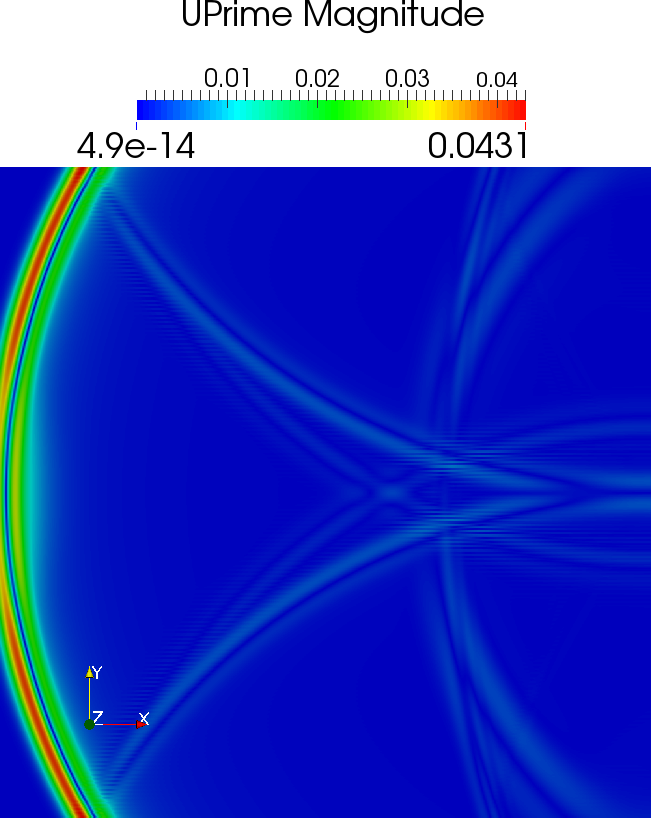
\includegraphics[keepaspectratio, width=0.49\columnwidth]{figures/acoustics1.png}
 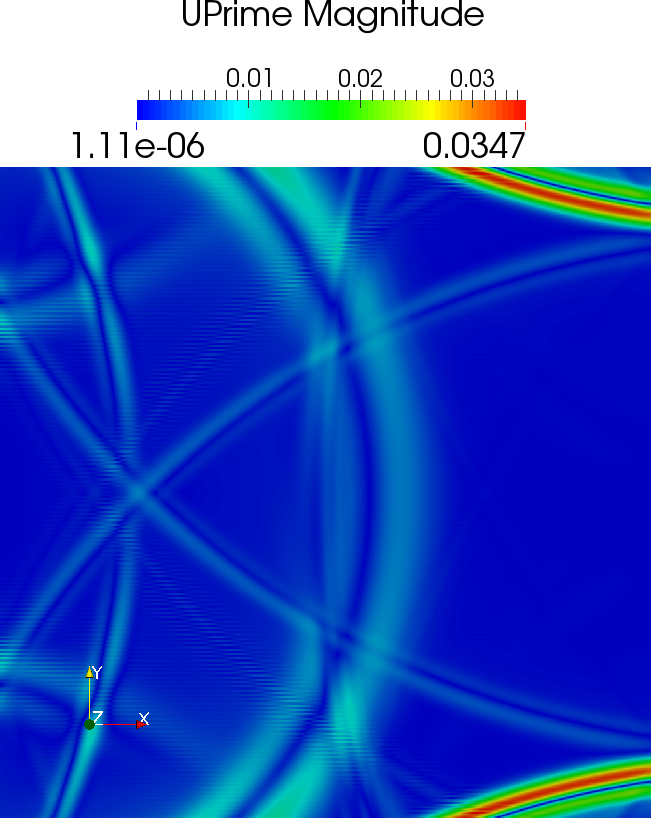
\includegraphics[keepaspectratio, width=0.49\columnwidth]{figures/acoustics2.png}
 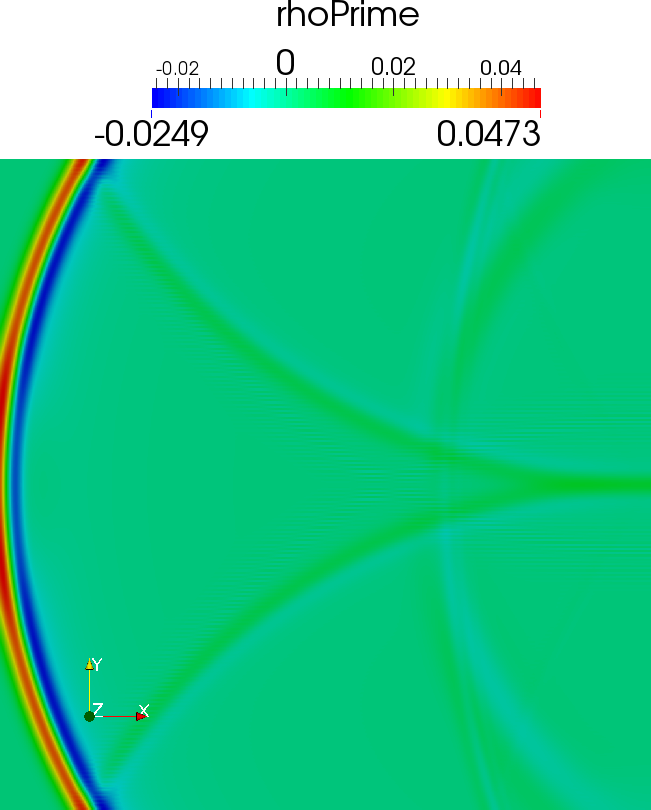
\includegraphics[keepaspectratio, width=0.49\columnwidth]{figures/acoustics3.png}
  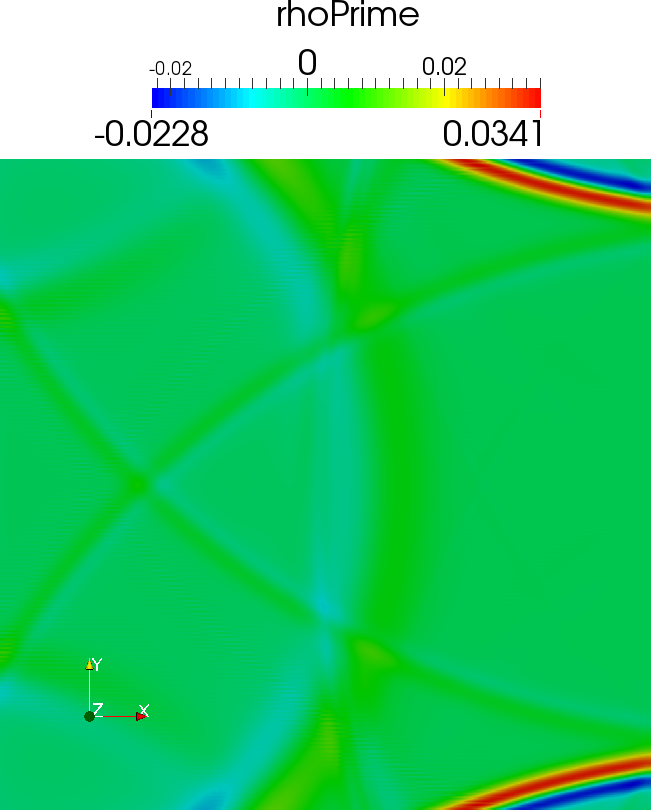
\includegraphics[keepaspectratio, width=0.49\columnwidth]{figures/acoustics4.png}
\small FVM simulations of flow induced noise, conducted by a Master student at FSB, Zagreb: velocity and density fluctuations in time.
\end{center}
}
\end{minipage}
}
\hspace{1cm}
%
% Second box
\begin{minipage}[t][79cm][t]{0.3\linewidth}
  % Title
  \vspace{0.5cm}
  % Main content: Adjust font size to \large, \Large or \LARGE as needed
  \large
  \textcolor{fsbBlue}{%
    \Large \bfseries
    Methodology
  }\\
The solution is represented by a function using a Legendre modal
\textit{polynomial basis} $\Phi = (\Phi_0,...,\Phi_{N_p-1})$. The solution can
then be expressed as a linear combination:
\begin{equation}
u(x) = \sum_{n=0}^{N_p-1}{\Phi_n(x)}\tilde{u}_n,
\nonumber
\end{equation}
where $\tilde{u}_n$ are solution variable \textit{weights on modal values}.
The solution is a
combination of polynomials of different degree: constant, linear,
parabolic...,
which are calculated using the hierarchical formula:
\begin{equation}
P_{n+1}(x) = \frac{1}{n+1}((2n+1) \cdot x P_n(x) - n \cdot P_{n-1}(x)).
\nonumber
\end{equation}
\begin{center}
 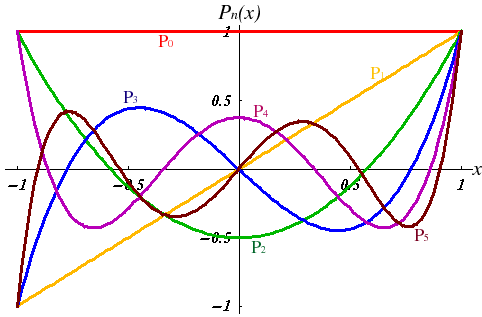
\includegraphics[keepaspectratio, width=0.99\columnwidth]{figures/LegendrePPlot.png}
\small Legendre polynomials up to 5\textsuperscript{th} degree.
\end{center}
The equations are written in a \textit{weak formulation}, i.e. finding the
solution of the system is equivalent to minimising the overall error (residual).
The error is minimised on the approximation (test) function space. We use the
\textit{Bubnov--Galerkin} approach, where the solution basis and test functions
are the same. The integration of surface and volume integrals over the cell and
the face is done with
\textit{Gaussian quadrature rule}. \\
  \large
  \textcolor{fsbBlue}{%
    \Large \bfseries
    \\Matrix support
  }\\
The system of equations to be solved can be written as:
\begin{align*}
\mathbf{M} \cdot \tilde{u} = \tilde{f}
\end{align*}
where $\mathbf{M}$ is a block--matrix: since the unknowns are represented using
polynomials of arbitrary degree, the dimensions of the matrix are $K \cdot N_p$,
where $K$ is the number of cells and $N_p$ is the order of the polynomial. The
support for block--systems in OpenFOAM is advanced and flexible, enabling easy
construction of block--matrices based on the face addressing from the
computational mesh. Also, an extensive library of block--linear solvers is
available in OpenFOAM, with the state--of--the--art multigrid solvers, namely
the selective algebraic multigrid, implemented by Jasak and Uroi\'{c}
(Computers\&Fluids, 2018).\\


\end{minipage}
%
\hspace{1cm}
% Third box
\begin{minipage}[t][79cm][t]{0.3\linewidth}
  % Main content: Adjust font size to \large, \Large or \LARGE as needed
  \large
%  \textcolor{fsbBlue}{%
%    \Large \bfseries
%    Example
%  }\\
Selective multigrid was tested with the implicitly--coupled incompressible turbulent flow solver and theoretical convergence of one order of magnitude per iteration was achieved for complex cases with highly unstructured meshes.
\begin{center}
 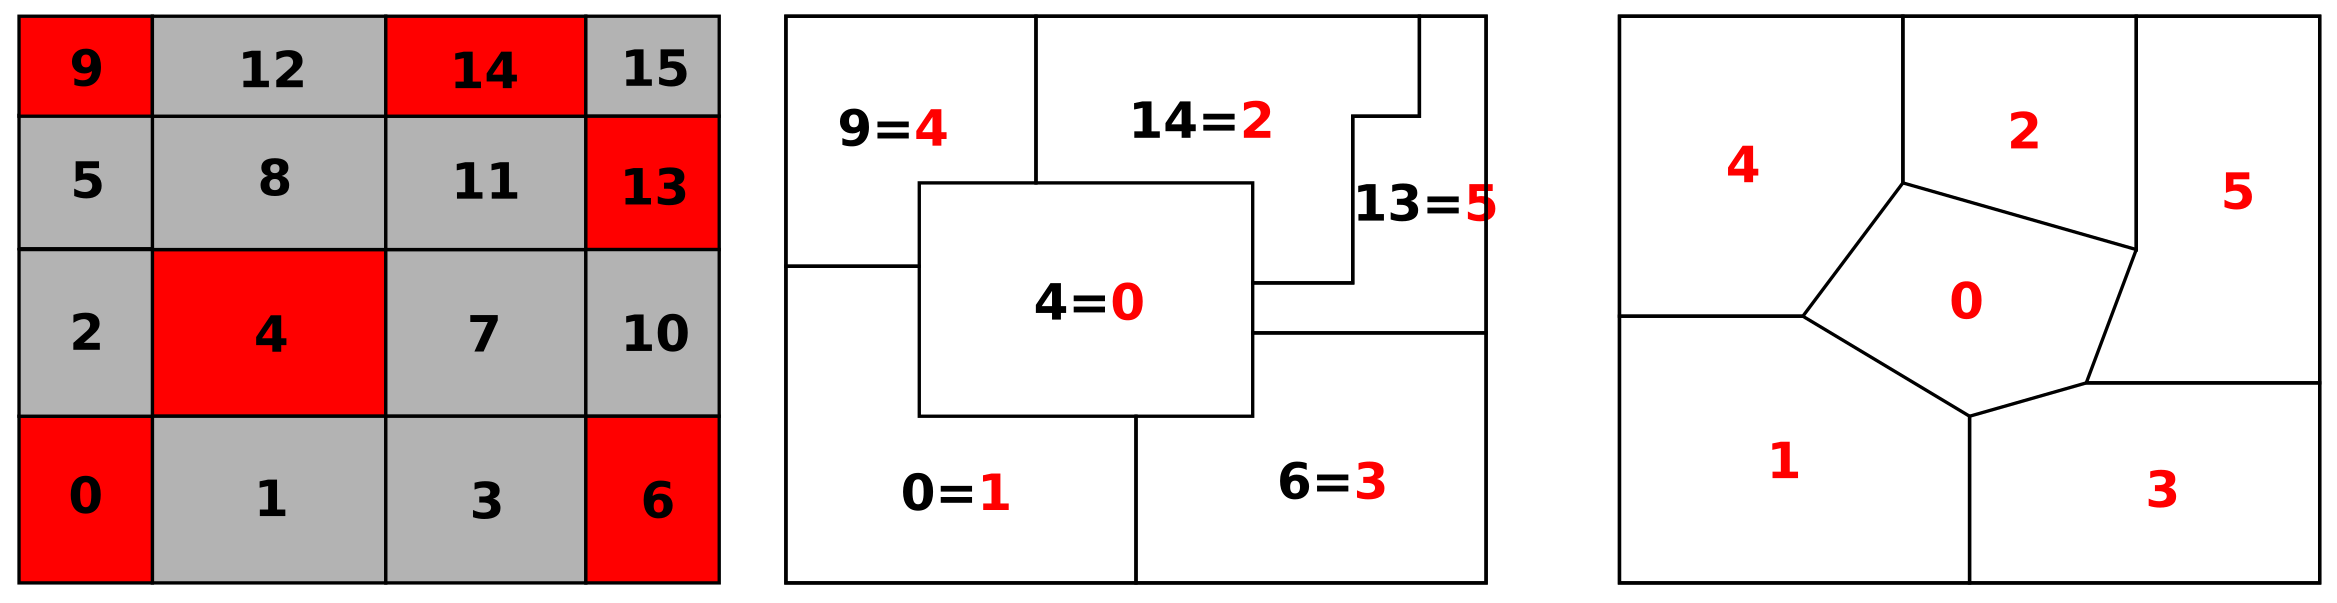
\includegraphics[keepaspectratio, width=0.99\columnwidth]{figures/polyhedra_SAMG.png}\\
 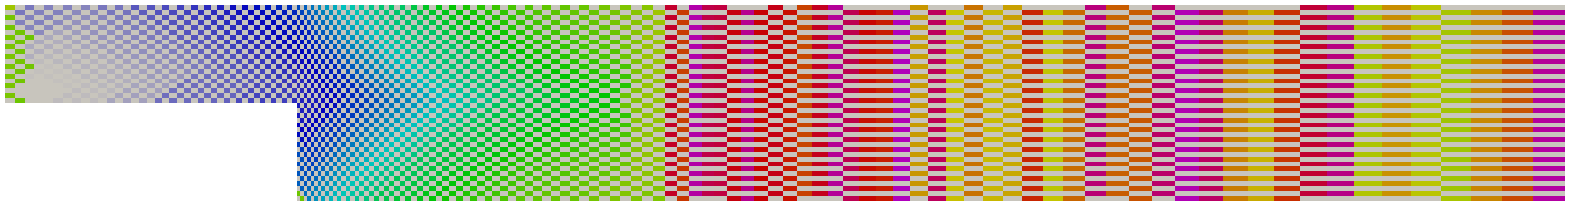
\includegraphics[keepaspectratio, width=0.99\columnwidth]{figures/time50_coarseningSAMG_level_0.png}\\
  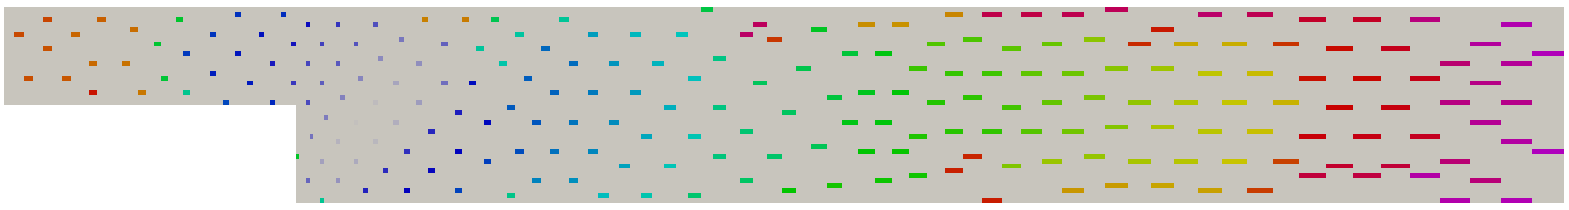
\includegraphics[keepaspectratio, width=0.99\columnwidth]{figures/time50_coarseningSAMG_level_2.png}\\
   
\includegraphics[keepaspectratio, width=0.99\columnwidth]{figures/time50_coarseningSAMG_level_5.png}
\small Example of creating coarse matrix levels in selective AMG.
\end{center}

  \large
  \textcolor{fsbBlue}{%
    \Large \bfseries
    \\Example - DG discretisation of a Laplacian
  }\\
We are assembling a linear system which is a discrete representation of the
following problem:
\begin{align*}
\begin{cases}
& \Delta u = \div (\grad u) = g_{\Omega} \, \text{ in $\Omega$} \\
& u = g_D \, \text{ on $\Gamma_D$, Dirichlet B.C.} \\
& \grad u \cdot n_{\partial \Omega} = g_N \, \text{ on $\Gamma_N$, Neumann B.C.}
\end{cases}
\end{align*}
It was shown that the system is \textit{consistent} and \textit{stable} if it
satisfies the coercitivity condition. Nitsche's method (1971), called Symmetric
Interior Penalty (SIP) is one possibility which satisfies this condition:
\begin{align*}
a_{SIP}&(u,v)
= \int_{\Omega} \underbrace{\grad u \cdot \grad v}_{\text{volume term - 1}}\ dV \\
 - &\oint_{\Gamma \setminus \Gamma_N} \underbrace{\{ \grad u\} \cdot n_\Gamma [|v|]}_{\text{consistency term - 2}} + \underbrace{\{ \grad v\} \cdot n_\Gamma [|u|]}_{\text{symmetry term - 3}}\ dA \\
 + &\oint_{\Gamma \setminus \Gamma_N} \underbrace{\eta [|u|][|v|]}_{\text{penalty term - 4}}\ dA
\end{align*}
\parbox{\textwidth}{
Here, term 2 ensures consistency. Term 3 is added for symmetry (and the method
is truly variational $\rightarrow$
the discrete solution minimizes $\frac{a(u,u)}{2} - \int g_{\Gamma}v\ dV$).
Thus, $a_{SIP}(-,-)$ is symmetric. The penalty term 4 guarantees
stability (Nitsche proved that if $\eta$ is taken as $C/h$, where $h$ is the
element size and $C$ a sufficiently large constant, discrete solution converges
to the exact solution with optimal order). It prevents spurious solutions by
controlling the gradients.
Considering that $a_{SIP}(-,-)$ is linear:}
\small
\begin{align*}
\underbrace{\begin{bmatrix}
a_{SIP}(\Phi^0_0, \Phi^0_0) & \hdots  & a_{SIP}(\Phi^{K - 1}_{N_p - 1}, \Phi^0_0) \\
\vdots & \vdots & \vdots \\
\vdots & \vdots & \vdots \\
a_{SIP}(\Phi^0_0, \Phi^{K - 1}_{N_p - 1}) & \hdots  & a_{SIP}(\Phi^{K - 1}_{N_p - 1}, \Phi^{K - 1}_{N_p - 1})
\end{bmatrix}}_{=: M_{SIP}} \cdot
\underbrace{\begin{bmatrix}
\tilde{u}^0_0\\
\vdots \\
\vdots \\
\tilde{u}^{K - 1}_{N_p - 1}
\end{bmatrix}}_{=: \tilde{u}} =
\underbrace{\begin{bmatrix}
\int g_{\Omega} \Phi^0_0\ dV\\
\vdots \\
\vdots \\
\int g_{\Omega} \Phi^{K - 1}_{N_p - 1}\ dV
\end{bmatrix}}_{=: \tilde{g}}
\end{align*}
\large
The unknowns are sorted in a cell--by--cell manner, to satisfy a
block--structure of $\mathbf{M}_{SIP}$.


\end{minipage}

%-------------------------------------------------------------------------------
%   TRANSITION FROM MAIN CONTENT TO FOOTER
%-------------------------------------------------------------------------------

\vspace{1.6cm}

%-------------------------------------------------------------------------------
%   POSTER FOOTER
%-------------------------------------------------------------------------------

\fcolorbox{fsbBlue}{fsbBlue}{%
\begin{minipage}[t][4cm][c]{0.3\linewidth}
  % Work Type
  \begin{center}
    \textcolor{white}{%
      \Large
      8th Floor CFD@FSB\\
      \vspace{0.5cm}% Spacing for neater formatting
      Zagreb, 2018\\
    }
  \end{center}
\end{minipage}
% Second box
\begin{minipage}[t][4cm][c]{0.7\linewidth}
  % Title
  \begin{center}
    \textcolor{white}{%
      \Large
      www.fsb.hr/cfd
    }
  \end{center}
\end{minipage}
}

%-------------------------------------------------------------------------------
%   Note
%-------------------------------------------------------------------------------

\begin{minipage}[t][0.6cm][c]{\linewidth}
  % Additional notes
  \begin{center}
      \vspace{0.8cm}
      \large
      Feel free to contact us at
      \href{mailto:cfd@fsb.hr}{cfd@fsb.hr}
      or take a look at our
      YouTube channel: 8th Floor CFD@FSB.
  \end{center}
\end{minipage}

\end{document}
